
\begin{paperappendix}
\section{}

\subsection{Notes on Sect. \ref{sec:LanguageSpecific}}\label{sec:PearsonResds}

%\subsection{Pearson distribution and Pearson residuals}

When dealing with categorical data as discussed in this chapter, we
typically want to know if two or more variables correlate. In other
words, we want to know if a property of some observation -- a level of
a variable -- allows us to make inferences about some other property
of that observation.
%
According to the null hypothesis (of statistical independence), which
says that the two variables are unrelated, the conditional probability
of observing a specific property $A$ in some observation $x$, given
some other property $B$ of $x$, is identical to the probability of
observing $A$ in $x$ independently of $B$ (cf. \bv{condprob}). Put
differently, the probability of any $x$ exhibiting both $A$ and $B$ is
the product of the probabilities of $A$ and $B$ (cf. \bv{conjprob}).

\begin{exe}
  \ex\label{indep} Assumption of independence:
  \begin{xlist}
    \ex\label{condprob} $p(A|B)=p(A)$
    \ex\label{conjprob} $p(A\wedge B) = p(A)\cdot p(B)$
  \end{xlist}
\end{exe}
%
If two variables do not correlate, the frequencies in a
contigency table will be proportional along both dimensions.
Consider Table \ref{tab:contingencyschema}.
%

\begin{table}[h]
  \begin{tabular}[h]{l|ll|l}
          &  A: level 1 & A: level 2 & $\Sigma$\\\hline
    B: level 1   &  a & b & a+b\\
    B: level 2   &  c & d & c+d\\\hline
    $\Sigma$ & a+c & b+d & a+b+c+d\\
  \end{tabular}
  \caption{Schematic contingency table}
    \label{tab:contingencyschema}
\end{table}

If the variables $A$ and $B$ are independent of each other, we expect
the ratio of any two pairs of cells $\frac{c_1}{c_2}$ and
$\frac{c_3}{c_4}$ to be the same if $c_1$ and $c_2$, and $c_3$ and
$c_4$, are in the same column, and $c_1$ and $c_3$, and $c_2$ and
$c_4$, are in the same row (including the marginal row and column
sums). For instance:

\begin{exe}
  \ex
  \begin{xlist}
    \ex $\frac{a}{c}=\frac{b}{d}$
    \ex $\frac{a}{a+c}=\frac{b}{b+d}$
    \ex $\frac{a}{c}=\frac{a+b}{a+b+c+d}$
    \ex $\frac{a}{b}=\frac{c}{d}$
    \ex $\frac{a}{a+b}=\frac{c}{c+d}$
    \ex\label{abcd} $\frac{a}{a+c}=\frac{a+b}{a+b+c+d}$
  \end{xlist}
\end{exe}
%
Based on such analogies, we expect the following count for cell $a$,
under the assumption of statistical independence of the variables. The
equation in \bv{ahat} follows from \bv{abcd} by multiplication with
$(a+c)$ (the symbol $\hat{\phantom{a}}$ on the $\hat{a}$ indicates that this variable
represents an expected value).

\begin{exe}
      \ex\label{ahat} $\hat{a}=\frac{(a+c)(a+b)}{a+b+c+d}$   
\end{exe}
%
The difference between the observed frequency $a$ and the expected
frequency $\hat{a}$ provides a way of determining
deviations from statistical independence.

In what follows we use the matrix formalism, which provides a compact
way of expressing and generalising the above example. $C$ represents
the original contingency table, and $\hat{C}$ corresponds to the
matrix of the expected frequencies as calculated from the independence
condition as stated in \ref{indep}.
%
The matrix of \textbf{Pearson residuals} is then calculated as:

\begin{exe}
  \ex Pearson residuals\\$R=(C-\hat{C})/\sqrt{\hat{C}}$
\end{exe}
%
The matrix
$\sqrt{\hat{C}}$ contains the square roots of the cells in
$\hat{C}$. Division by the square root of the expected value is a
standardization step. We assume Poisson sampling (independent
selection of subjects), so each cell is assumed to follow a Poisson
distribution. In a Poisson distribution, the variance is equal to the
expected value (both values are represented by the parameter
$\lambda$). We divide the difference between the expected and the
observed value by the square root of the variance -- the standard
deviation -- to standardize the values.

In matrix notation, the matrix of expected values $\hat{C}$ can be
represented as follows:

\begin{exe}
  \ex\label{PearsonDef}
  \begin{xlist}
    %\ex $R=(C-\hat{C})/\sqrt{\hat{C}}$,
    \ex $\hat{C}=(m_m\otimes m_n)/N$, (the outer product of row and
    column margins, divided by the number of
    observations) %$\sum_{0=1}^m\sum_{0=1}^nC_{m,n}\times m_m\otimes
                  %m_n$,
    \ex   $m_m=1C, m_n=1C^\mathsf{T}$, (row and column sums)
    \ex   $N=1^\mathsf{T} C1$ (the sum of all cells)
  \end{xlist}
  %$m_m$ and $m_n$ being the row and column masses, respectively.  
\end{exe}
%
The \textbf{adjusted Pearson residuals} are obtained 
as shown in \bv{adjresid}. We divide the difference between the
observed and the expected value by an estimate of the standard error
based on the assumption that the marginal sums are fixed, therefore
assuming a hypergeomteric distribution. Adjusted Pearson residuals are
always larger than unadjusted Pearson residuals, as the additional
term in the demoninator -- $\sqrt{(1-m_m/N)(1-m_n/N)}$ -- is always
smaller than 1.

\begin{exe}
  \ex\label{adjresid} $\tilde{r}=\frac{C-\hat{C}}{\sqrt{\hat{C}(1-m_m/N)(1-m_n/N)}}$
\end{exe}

\subsection{Notes on ordination}\label{sec:AppOrdination}

The information in this section is mainly intended to facilitate an
intuitive understanding of the methods. For more complete and more
accurate information, please consult \citet{Greenacre2016}.

\subsubsection*{Some terms and concepts}

A \textbf{contingency table} is a table with counts of observations
with specific properties, cf. Table \ref{tab:contingency}.

\begin{table}[ht]
\centering
\begin{tabular}{r|rrr|r}
  \hline
 & comm & dir.boul & repr & $\Sigma$\\ 
  \hline
  \textit{gleich}       &   4 &   3 &  18 & 25      \\ 
  \textit{sofort}       &   2 &  14 &  18 & 34\\ 
  \textit{unverzüglich} &   1 &   6 &   2 & 9 \\\hline
  $\Sigma$       &   7 &  23 &  38 & 68 \\
   \hline
\end{tabular}
\caption{Contingency table}
\label{tab:contingency}
\end{table}

A \textbf{percentage table} shows the relative frequency of each cell,
i.e., the cell value divided by the number of observations (cf. Table
\ref{tab:percentage}).  The \textbf{row} and \textbf{column masses}
(the margins of Table \ref{tab:percentage}) are the relative
frequencies of all observations in specific rows or columns.

\begin{table}[hb]
\centering
\begin{tabular}{r|rrr|r}
  \hline
 & comm & dir.boul & repr & $\Sigma$\\ 
  \hline
  \textit{gleich} & 0.06 & 0.04 & 0.26 & \textbf{0.37}\\ 
  \textit{sofort} & 0.03 & 0.21 & 0.26 & \textbf{0.50}\\ 
  \textit{unverzüglich} & 0.01 & 0.09 & 0.03 & \textbf{0.13}\\ 
  \hline
  $\Sigma$               & \textbf{0.11}   & \textbf{0.34}    &  \textbf{0.56}   &    1\\
\end{tabular}
\caption{Percentage table}
\label{tab:percentage}
\end{table}

The \textbf{profile} of a given category constituting the row of a
contingency or percentage table is the rowwise proportion of that
category (cf. Table \ref{tab:profile}).

\begin{table}[ht]
\centering
\begin{tabular}{r|rrr|r}
  \hline
 & comm & dir.boul & repr & $\Sigma$\\ \hline
  \textit{gleich} & 0.16 & 0.12 & 0.72 & 1\\ 
  \textit{sofort} & 0.06 & 0.41 & 0.53 & 1\\ 
  \textit{unverzüglich} & 0.11 & 0.67 & 0.22 & 1\\ \hline
\end{tabular}
\caption{Row profiles}
\label{tab:profile}
\end{table}

The \textbf{average profile} -- geometrically speaking the
\textbf{centroid} -- is the average of the row profiles, weighted by
the row masses. For the first column:

 \begin{exe}
   \ex $\hat{c_1} = 0.37 \cdot 0.16 + 0.5 \cdot 0.06 + 0.13 \cdot 0.11 = 0.1$
 \end{exe}
%
 The average profile for Table \ref{tab:contingency} is thus:

 \begin{exe}
   \ex $\hat{C}_{j+} = (0.1\; 0.34\; 0.56)$
 \end{exe}
%
 We can obtain a \textbf{standardized profile table} by scaling the columns of
 the profile table (Table \ref{tab:profile}) by the inverse of the
 square root of the average profile values (i.e., we divide each value
 by the square root of the corresponding average profile value).
 For example, the average profile value of the first column is $0.1$,
 and its square root is $\approx 0.32$. If we divide $0.16$ (the first
 value of the profile of \textit{gleich}) by $0.32$, we obtain a value of
 $0.5$:

\begin{table}[ht]
\centering
\begin{tabular}{rrrr}
  \hline
 & 1 & 2 & 3 \\ 
  \hline
  gleich & 0.5 & 0.21 & 0.96 \\ 
  sofort & 0.18 & 0.71 & 0.71 \\ 
  unverzüglich & 0.35 & 1.15 & 0.30 \\ 
   \hline
\end{tabular}
\caption{Standardized profile table}
\end{table}
%
In a coordinate system scaled by the inverse of the square root of the expected
value Euclidean distances are equivalent with Chi-squared distances.

The \textbf{Chi-squared distance} $\chi^2_{\Delta}$ is the square root
of the sum of the squared differences between the observed values and
the expected values, divided by the expected values.
%
For each row $m$ of a matrix $C_{m\times n}$:
\begin{exe}
  \ex
  $\chi^2_{\Delta,m} =
  \sqrt{\sum_{i=1}^{n}{\frac{(C_{m,i}-\hat{C}_{m,i})^2}{\hat{C}_{m,i}}}}$

  ($\hat{C}$ being the matrix of expected values, see (\ref{PearsonDef}))

\end{exe}
%
The sum of the Chi-squared distances of a matrix provides the basis
for the concept of \textbf{inertia} in Correspondence Analysis. The
inertia of a contingency table is %the weighted average of the
% Chi-square distances of each row to the row profile, where the average
% is weighted by the row masses $M$
``the weighted average of the squared $\chi^2$ -distances between the
row profiles and their average profile'' \citep[29]{Greenacre2016}. It is 
weighted by the row masses $M$.
For a matrix  $C_{m\times n}$,

\begin{exe}
  \ex $I_C=\sum_{i=1}^m\sum_{j=1}^nM_i\frac{(C_{i,j}-\hat{C}_{i,j})^2}{\hat{C}_{i,j}}$.
\end{exe}
%
Note that the Chi-squared distance is identical to the Chi-squared
value of a table, divided by the number of observations, and that it
is equivalent to the $\phi$-coefficient squared, so
$\phi=\sqrt{\chi^2/n}$.

\subsubsection*{Singular value decomposition}\label{sec:SVD}

As a starting point of singular value decomposition,
we use a table of standardized residuals. It is
obtained just as was in described in Sect. \ref{sec:PearsonResds} for the
Pearson residuals. However, in Correspondence Analysis we calculate
standardized residuals from a percentage table as shown in Table
\ref{tab:percentage}, not from a contingency table as shown in Table
\ref{tab:contingency}. The two tables differ by a factor of
$\sqrt{N}$, i.e., in our case, $8.246$ (=$\sqrt{68}$). Table
\ref{tab:StandResds} contains standardized residuals.

\begin{table}[ht]
\centering
\begin{tabular}{rrrr}
  \hline
                        & comm & dir.boul & repr \\ 
   \hline
  \textit{gleich}       & 0.11 & -0.23 & 0.13 \\ 
  \textit{sofort}       & -0.10 & 0.09 & -0.03 \\ 
  \textit{unverzüglich} & 0.01 & 0.21 & -0.16 \\ 
   \hline
\end{tabular}
\caption{Table of standardized residuals}
\label{tab:StandResds}
\end{table}



\begin{figure}[t]
  \centering
  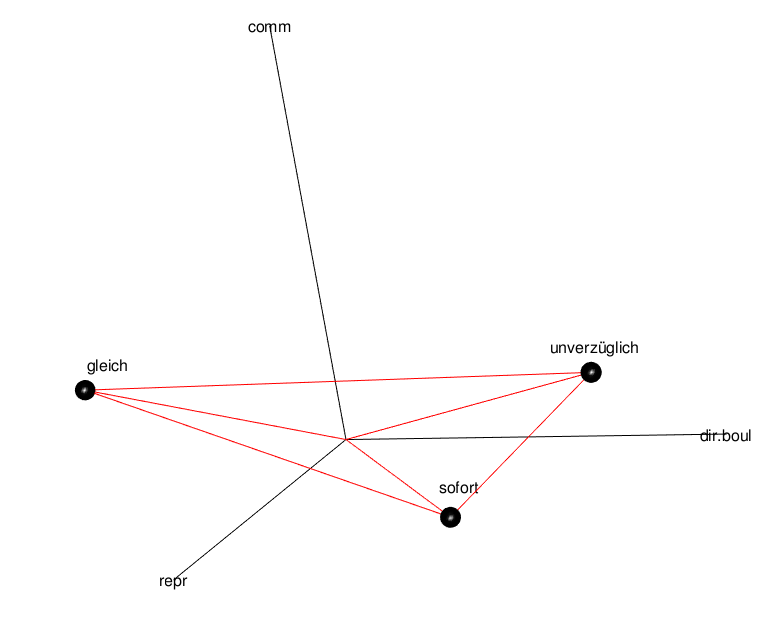
\includegraphics[width=0.5\linewidth]{figures/Ordination3b.png}
  \caption{Visualizing the standardized residuals of Table \ref{tab:PropTable}}
  \label{fig:Ordination3App}
\end{figure}

We can represent Table \ref{tab:StandResds} in a three-dimensional
coordinate system as shown in Figure \ref{fig:Ordination3} in the main
text, which is repeated for convenience in Figure
\ref{fig:Ordination3App}.
%
Alternatively, we can think of Table \ref{tab:StandResds} as a mapping
from one three-dimensional coordinate system to another three-dimensional
coordinate system. Let us assume a source system that consists of three unit
vectors only, i.e., a standard basis (cf. Figure
\ref{fig:Ordination3App}). When regarded as a transformation map,
Table \ref{tab:StandResds} (via matrix multiplication) maps the
standard basis to the residuals shown in red in Figure \ref{fig:Ordination4App}. What matters here is
that by regarding the matrix as a transformation map we can not only
map the three standard vectors to new coordinates, we can map
\textit{any} point in the source system to the target system. For example,
the point located at $(0.5\; 0\; 0)$, which is halfway between the
origin and the unit vector $(1\; 0\; 0)$ in the original system, will be
mapped to a point that is halfway between the origin and the target
vector of $(1\; 0\; 0)$ in the new system (see the two orange points
in Figure \ref{fig:Ordination4App}).

\begin{figure}[t]
  \centering
  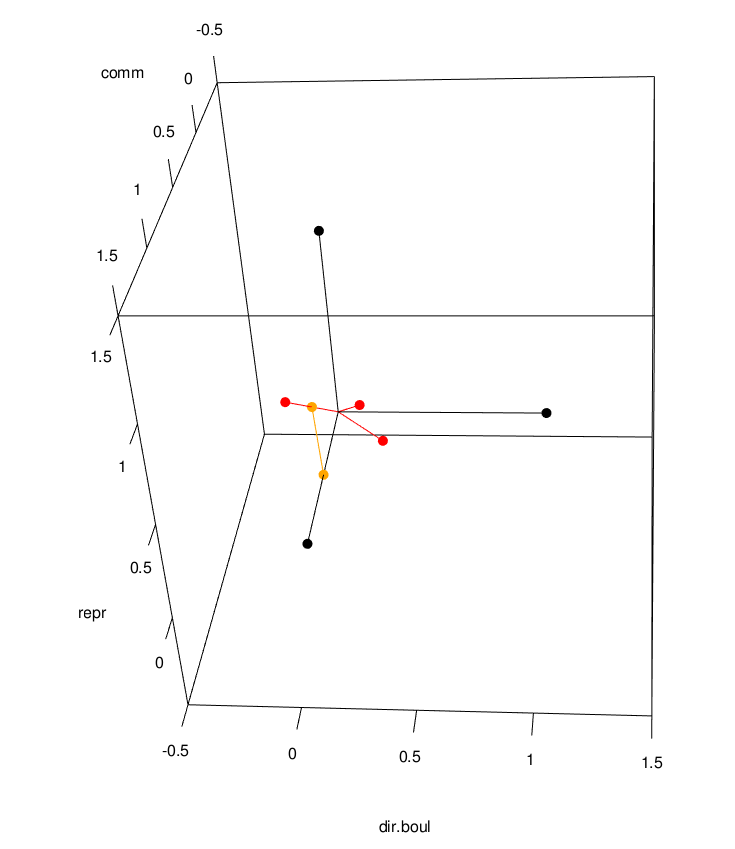
\includegraphics[width=0.5\linewidth]{figures/SVD3.png}
  \caption{Table \ref{tab:StandResds} as a mapping from a standard basis to a new coordinate system}
  \label{fig:Ordination4App}
\end{figure}

Under the transformation view of the matrix in Table
\ref{tab:StandResds} we can perform a `global' transformation of the
original coordinate system. Consider Figure \ref{fig:Sphere}, which shows a random
sample of vectors (represented as points) of unit length.  The cloud
of points shown in Figure \ref{fig:Sphere} can be mapped to the space
of standardized residuals in the same way in which we mapped the three
unit vectors to that space in Figure \ref{fig:Ordination3App} with
matrix multiplication. All points will be mapped to a `disc' that
contains the origin, see Figure \ref{fig:Ellipse}.

\begin{figure}[t]
  \centering
  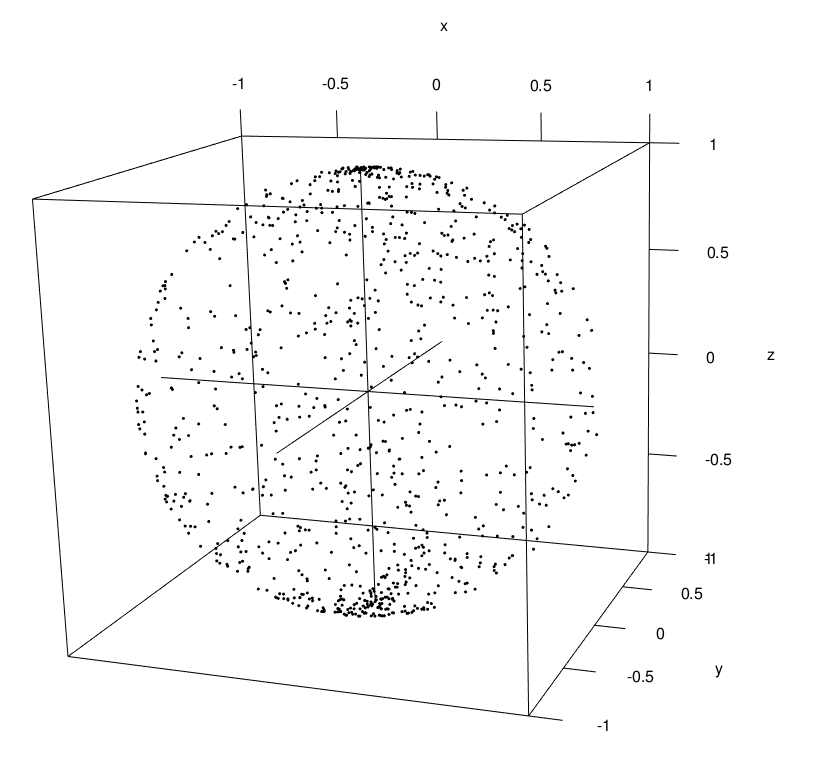
\includegraphics[width=0.5\linewidth]{figures/SVD4.png}
  \caption{A random sample of 1,000 vectors of length 1}
  \label{fig:Sphere}
\end{figure}


\begin{figure}[b]
  \centering
  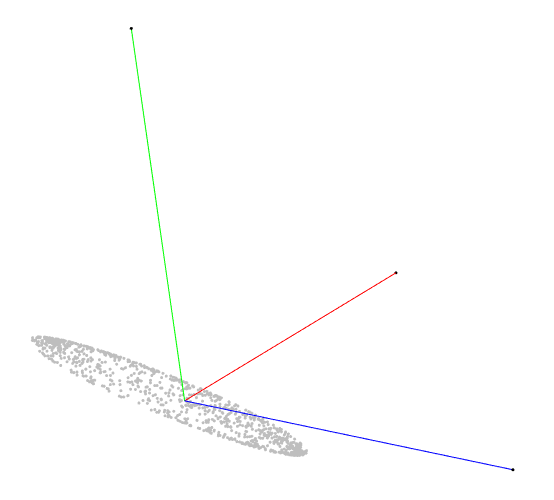
\includegraphics[width=0.5\linewidth]{figures/SVD5.png}
  \caption{The random sample of 1,000 vectors from Figure
    \ref{fig:Sphere} mapped to residual space}
  \label{fig:Ellipse}
\end{figure}

\pagebreak

We can now look at the `disc' of Figure \ref{fig:Ellipse} from a
different point of view, see Figure \ref{fig:Ellipse2}. This plot
shows two straight lines. The horizontal line points in the
direction in which the points of the new cloud are spread out most. It
is the first \textbf{singular vector}. The vertical line is orthogonal to the
horizontal line. It shows the direction in which the data is spread
out most, on the condition of being orthogonal to the first
line. (Note that there appears to be only one line that is orthogonal
to the first line, but remember that the disc is actually located in
three-dimensional space [see Figure \ref{fig:Ellipse}], so there are in
fact an infinite number of vectors that are orthogonal to the first
singular vector, pointing away from the disc).

\begin{figure}[t]
  \centering
  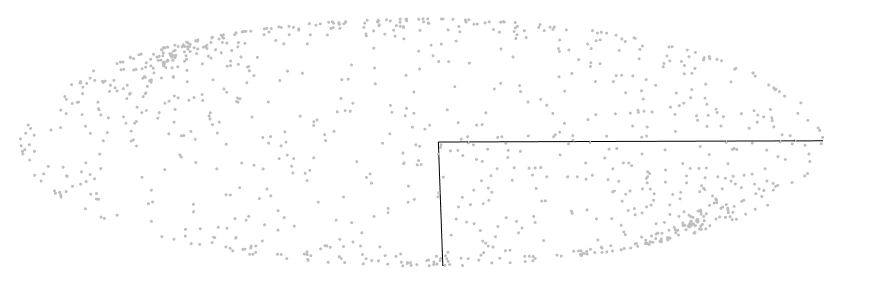
\includegraphics[width=0.5\linewidth]{figures/SVD6.png}
  \caption{The random sample of 1,000 vectors from Figure
    \ref{fig:Sphere} mapped to residual space, from a different perspective and with singular vectors}
  \label{fig:Ellipse2}
\end{figure}

Singular value decomposition is a method to find singular vectors and their lengths, the singular values.
It decomposes a matrix $M$ into two
square matrices $U$ and $V$ and a (rectangular diagonal) scaling matrix $\Sigma$ such
that:

\begin{exe}
  \ex\label{SVDFormula}  $M = U\Sigma V^*$
\end{exe}
%
where $^*$ denotes the conjugate transpose of a matrix. For matrices
of the type dealt with in the present context, the conjugate transpose
is identical to the transpose, i.e., $V^*=V^\mathsf{T}$.

The matrices $U$ and $V$ contain orthonormal bases as row and column vectors,
which means that these vectors are orthogonal to each other, and each vector is
of unit length. In the case of $U$, the row vectors are orthogonal, in
the case of $V$, it is the column vectors that are orthogonal, hence:

\begin{exe}
  \ex  $UU^T=I$
  \ex $V^TV=I$
\end{exe}
%
In our case, the SVD delivers the following
factorization (obtained with the function \verb+svd+ in R):

\begin{exe}
  \ex $U$ \hspace{3.7cm} $\Sigma$ \hspace{3.1cm} $V$
%\end{exe}

$\begin{bmatrix}
  -0.72 & 0.35 & 0.61 \\ 
   0.28 & -0.65 & 0.71 \\ 
   0.64 & 0.68 & 0.36 \\
\end{bmatrix}$
%
\hspace{1em}
  $\begin{bmatrix}
   0.39 & 0.00 & 0.00 \\ 
   0.00 & 0.12 & 0.00 \\ 
   0.00 & 0.00 & 0.00 \\ 
 \end{bmatrix}$
%
\hspace{1em}
%
  $\begin{bmatrix}
   -0.25 & 0.91 & -0.32 \\ 
   0.81 & 0.02 & -0.58 \\ 
    -0.52 & -0.41 & -0.75 \\
    \end{bmatrix}$
 \end{exe}
%
 To see that the first two row vectors of U are orthogonal (they stand in a $90^o$ angle to each other), consider their
 dot product:

 \begin{exe}
   \ex $u_1\cdot u_2$ \\
   $=(-0.715 \cdot 0.285) + (0.348 \cdot -0.647) + (0.606 \cdot 0.707)$\\
   $=-0.204 -0.225 + 0.429 = 0$
 \end{exe}
%
 To see that the length of the first vector is 1:

 \begin{exe}
   \ex $\sqrt{-0.715^2 + 0.348^2 + 0.606^2}$\\
   $=\sqrt{0.511 + 0.121 + 0.367}$\\
   $=\sqrt{1} = 1$
 \end{exe}
%
 The rows of $U$, and the columns of $V$, constitute the bases for the coordinates of the rows and columns in CA.
 %
 Both matrices are scaled by the inverse of the square root of the average profile values ($W_m, W_n$ below).
 %
 The matrix of interest is moreover scaled by the singular values in matrix $\Sigma$.
 %
 If we want to locate rows in a coordinated system defined by their associations with columns, we
 will only scale the left singular values, i.e., matrix $U$, by $\Sigma$.
 %
 If we want to locate columns in a coordinate system defined by their associations with rows, we scale the right singular values, i.e., matrix
 $V$, by $\Sigma$. Sets of coordinates, here represented as $C$, can thus be
 obtained as follows (in the text we were only interested in the row
 analysis):
 
 \begin{exe}
   \ex row analysis
   \begin{xlist}
   \ex $C_{row}= W_m U \Sigma$
   \ex $C_{col} = W_n V$     
   \end{xlist}
   \ex column analysis
     \begin{xlist}
   \ex $C_{col}= W_n V \Sigma$
   \ex $C_{row} = W_m U$     
   \end{xlist}
 \end{exe}
%
In an asymmetric map, where rows are represented in principal
coordinates and columns in standard coordinates, we can reconstruct
the original matrix from the map via the inner product between row and column
vectors. For example, the \ipadv\ \textit{gleich} and the column
`repr' have the following coordinates:

\begin{exe}
  \ex \textit{gleich}: $(-0.46\; 0.07)$
  \ex `repr': $(-0.70 -\!0.54)$ 
\end{exe}
%
These coordinates first need to be scaled by the square root of the row masses/average profile (to `undo' the scaling that was applied previously):

\begin{exe}
  \ex \textit{gleich}: $0.606\; (-0.463\; 0.067) = (-0.281\; 0.041)$
  \ex `repr': $0.748\; (-\!0.702\; -\!0.545) = (-\!0.525\; -\!0.407)$
\end{exe}
%
The inner product of these vectors is:

\begin{exe}
  \ex $-0.281\cdot -\!0.525 + 0.041\cdot -\!0.407=0.131$
\end{exe}
%
The result, $0.131$, is the standardized residual of the cell for \textit{gleich} and `repr'. 

\subsection{Notes on Sect. \ref{sec:ComparativeUndirected}}\label{sec:AppComparativeUndirected}

Figure \ref{fig:Silhouette} shows the silhouette plot for the
clustering reported on in Sect.  \ref{sec:ComparativeUndirected}.

\begin{figure}[h]
  \centering
  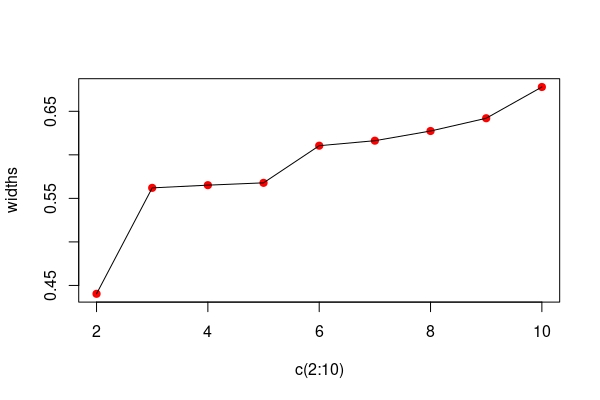
\includegraphics[width=0.5\linewidth]{figures/silhouette.jpeg}
  \caption{Silhouette widths for cluster solutions}
  \label{fig:Silhouette}
\end{figure}


%\subsection{Notes on Sect. \ref{sec:GraphicalModels}}\label{sec:AppGraphicalModels}



%\section{Notes on the chi-squared test}


%\section{Notes on ordination}







%%% Local Variables:
%%% mode: latex
%%% TeX-master: "main"
%%% End:
\end{paperappendix}
